%%%%%%%%%%%%%%%%%%%%%%%%%%%%%%%%%%%%%%%%%
% CN2 Labreport template
%
% License:
% CC BY-NC-SA 3.0 (http://creativecommons.org/licenses/by-nc-sa/3.0/)
%
%%%%%%%%%%%%%%%%%%%%%%%%%%%%%%%%%%%%%%%%%

\documentclass[parskip=full]{scrartcl}

\usepackage{siunitx}  % Provides the \SI{}{} command for typesetting SI units
\usepackage{graphicx} % Required for the inclusion of images
\usepackage{booktabs} % nicer tables
\usepackage[noabbrev]{cleveref} % automatic references
\usepackage{listings} % typeset code

\crefname{lstlisting}{listing}{listings} % for referencing code
\Crefname{lstlisting}{Listing}{Listings} % for referencing code

\usepackage[headsepline]{scrlayer-scrpage} % header
\ohead{Group 08} % right part of header
\ihead{Assignment 2} % left part of header

\lstset{basicstyle=\ttfamily} % monospaced font in listing

\usepackage{lstautogobble}  % Fix relative indenting
\usepackage{color}          % Code coloring
\usepackage{zi4}            % Nice font

\definecolor{bluekeywords}{rgb}{0.13, 0.13, 1}
\definecolor{greencomments}{rgb}{0, 0.5, 0}
\definecolor{redstrings}{rgb}{0.9, 0, 0}
\definecolor{graynumbers}{rgb}{0.5, 0.5, 0.5}

\usepackage{listings}
\lstset{
    autogobble,
    columns=fullflexible,
    showspaces=false,
    showtabs=false,
    breaklines=true,
    showstringspaces=false,
    breakatwhitespace=true,
    escapeinside={(*@}{@*)},
    commentstyle=\color{greencomments},
    keywordstyle=\color{bluekeywords},
    stringstyle=\color{redstrings},
    numberstyle=\color{graynumbers},
    basicstyle=\ttfamily\footnotesize,
    frame=l,
    framesep=12pt,
    xleftmargin=12pt,
    tabsize=4,
    captionpos=b
}


%----------------------------------------------------------------------------------------
%	DOCUMENT INFORMATION
%----------------------------------------------------------------------------------------

\begin{document}
\begin{titlepage}
    \centering
    \vspace*{2cm}
    {\Huge \textbf{Communication Networks 2}}\\
    SS 2019\\
    \vspace*{1cm}
    {\Large Assignment 2}
    \\\vspace*{3cm}
    {\Large \textbf{Group 08}}\\
    \vspace*{1cm}
    {\large 
        \begin{tabular}{l c c}
            Name & Mat.Nummer \\ \hline
            Constantin SCHIEBER & 01228774 \\
            Andreas HIRTENLEHNER & 01327273
        \end{tabular}
    }
    \\\vspace*{7cm}
    \today
\end{titlepage}

%----------------------------------------------------------------------------------------
%	SECTION 1
%----------------------------------------------------------------------------------------
\section{Description of the Solution}
Linphone was used and configured to register with the provided SIP Registrar (Figure \ref{fig:registerLinphone}).
The provided SIP identity and password were used (\texttt{sip:cn\_08@cn2lab.cn.tuwien.ac.aut}) for this (Figure \ref{fig:registerLinphone} shows the setup dialouge).
\begin{figure}[ht]
    \centering
   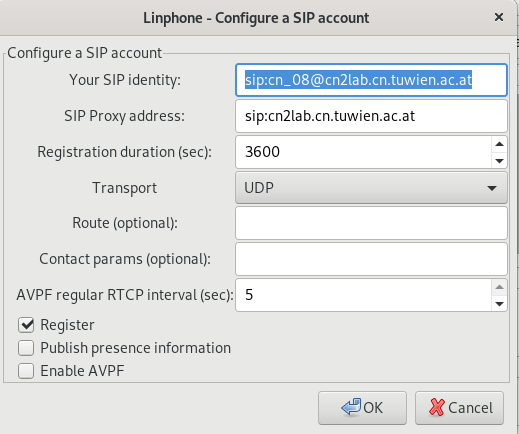
\includegraphics[width=0.5\textwidth]{images/linphoneSettings.png} 
    \caption{Setup of the Linphone client}
    \label{fig:registerLinphone}
\end{figure}

\subsection{Secret Message to the Registrar}
A Wireshark log was created to detect the secret message to the registrar.
A filter for \texttt{SIP} was set up to observe the communication between the Registrar and our client.
We look for registration operations which enable the server to know the location of our client.
For this purpose, REGISTER messages are exchanged in a regular interval and the Registrar associates our SIP identity with our currently used machine (for a detailed description refer to RFC 3261, p. 16 and the lecture slides CN2-05-SIP, p. 103).
The \texttt{secret-message} field that is to be found is an unrecognised SIP header that does not conform to the standards of the protocol.
It is present in the header of \texttt{200 OK} messages that are sent by the server and has the value \texttt{Dohugiwiqi3}, which is the secret message.
Our tutor confirms that the \texttt{secret-message} field is indeed purposely inserted for this lecture and does not have any further meaning.
\begin{figure}[ht]
    \centering
   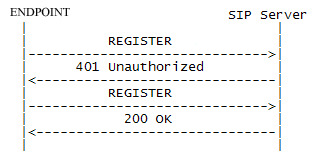
\includegraphics[width=0.5\textwidth]{images/sip_register_flow.jpg} 
    \caption{SIP Register Flow (https://www.voipmechanic.com/sip-call-example.htm)}
    \label{fig:sipRegisterFlow}
\end{figure}
\subsection{Discussion of Measured Network Parameters}
Factors that influence Quality of Service (QoS) include available bandwidth, latency, packet loss, packet delay variation, out-of-order delivery and rate of corrupted packets. 
With Wireshark (under \texttt{Telephony > RTP > Show all streams}), we analysed lost packets, the delta between packets and the jitter (as RTP packets contain information on the senders time).
Table \ref{tbl:rtpStatistics} shows these statistics for both servers.
They confirm our subjective observation that Landline provides a better QoS than Satellite.
The call with Landline has zero lost packets while Satellite looses between 4-5\% of its packets which may result in digital artefacts. 
A higher mean jitter for Satellite means that a bigger playback buffer is required, which results in a degradation of real-time capabilities or a stuck video stream. %TODO: Verify this statement?)
While a jitter of 30ms already leads to quality degradation of the service it is becoming unacceptable at over 100ms (\cite{noauthor_voip_2015}, \cite{noauthor_voip_2016}).

%TODO: Remove Max Delta and Max Jitter values?
\begin{table}
    \centering
    \begin{tabular}{c c c c c c c}
       \hline
       Server & Payload & Packets & Lost (\%) & Max Delta (ms) & Max Jitter (ms) & Mean Jitter (ms)\\
       \hline
       Landline & VP8 & 1553 & 0\% & 128 & 10.7 & 1.1 \\
       Landline & opus & 497 & 0\% & 43 & 7.8 & 4.9 \\
       Satellite & VP8 & 2280 & 4.5\% & 103 & 7.45 & 3.14\\
       Satellite & opus & 589 & 5.3\% & 68 & 19.4 & 14.2\\
       \hline
    \end{tabular}
    \caption{Wireshark RTP statistics for the two servers}
    \label{tbl:rtpStatistics}
\end{table}

% Useful links: 
% - https://osqa-ask.wireshark.org/questions/48014/how-can-i-measure-packet-loss-delay-and-jitter-for-a-streaming-video-over-a-lan
% - https://osqa-ask.wireshark.org/questions/52294/how-can-i-measure-throughput-packet-loss-delay-and-jitter-for-a-streaming-video-over-wifi
% - https://osqa-ask.wireshark.org/questions/29008/what-are-difference-and-delta-in-wireshark-rtp-analysis

\subsection{Discussion of subjective QoS}
We compared three different codecs for subjective video and sound quality.
As expected, a changed codec for the Landline connection does not make any difference in the subjective QoS.
This is because a good connection will deliver good results, even if the codec is not highly efficient / optimized (after all, the codec is designed to work as expected, at least under optimal conditions).

MP4V-ES (MPEG4, Part 2) is a codec that integrates with H.263, a standard that is optimized towards usage with a low available bandwidth ($<$ 64kbit/s).
It heavily uses temporal compression, i.e. works best when there is a low amount of movement between frames.
Since H263-1998 only provides additional optional features and therefore should come out very similar to H.263.

% Useful links:
% - https://linphone-developers.nongnu.narkive.com/fpQKrGMb/difference-between-video-profiles-mp4v-es-and-h264
\begin{itemize}
	\item Landline, Opus, VP8: 5 (very good quality)
	\item Satellite, Opus, VP8: 3 (slight cracking in audio, video freezing every 5s)
	\item Satellite Speex, MP4V-ES: bad quality, fragments in picture but no freezes, lag
	\item Landline Speex, MP4V-ES: No difference in quality
	\item Satellite H263-1998, PCMU: bad quality, smoother fragments in picture but no freezes, lag
	\item Landline H263-1998, PCMU: No difference in quality
\end{itemize}

\section{QoS Analysis}
To compare the two server connections and the different codecs, especially in low peformance networks, plots of different packet parameters generated by Wireshark (\texttt{Telephony -> RTP Streams}) were made. 
Figure \ref{fig:vp8_jitter} shows the jitter for both server connections. 
It is clearly evident from the histogram and the CDF, that packets coming from the Landline server have more jitter than from the Satellite server, which results in a worse QoS.

\begin{figure}
    \centering
    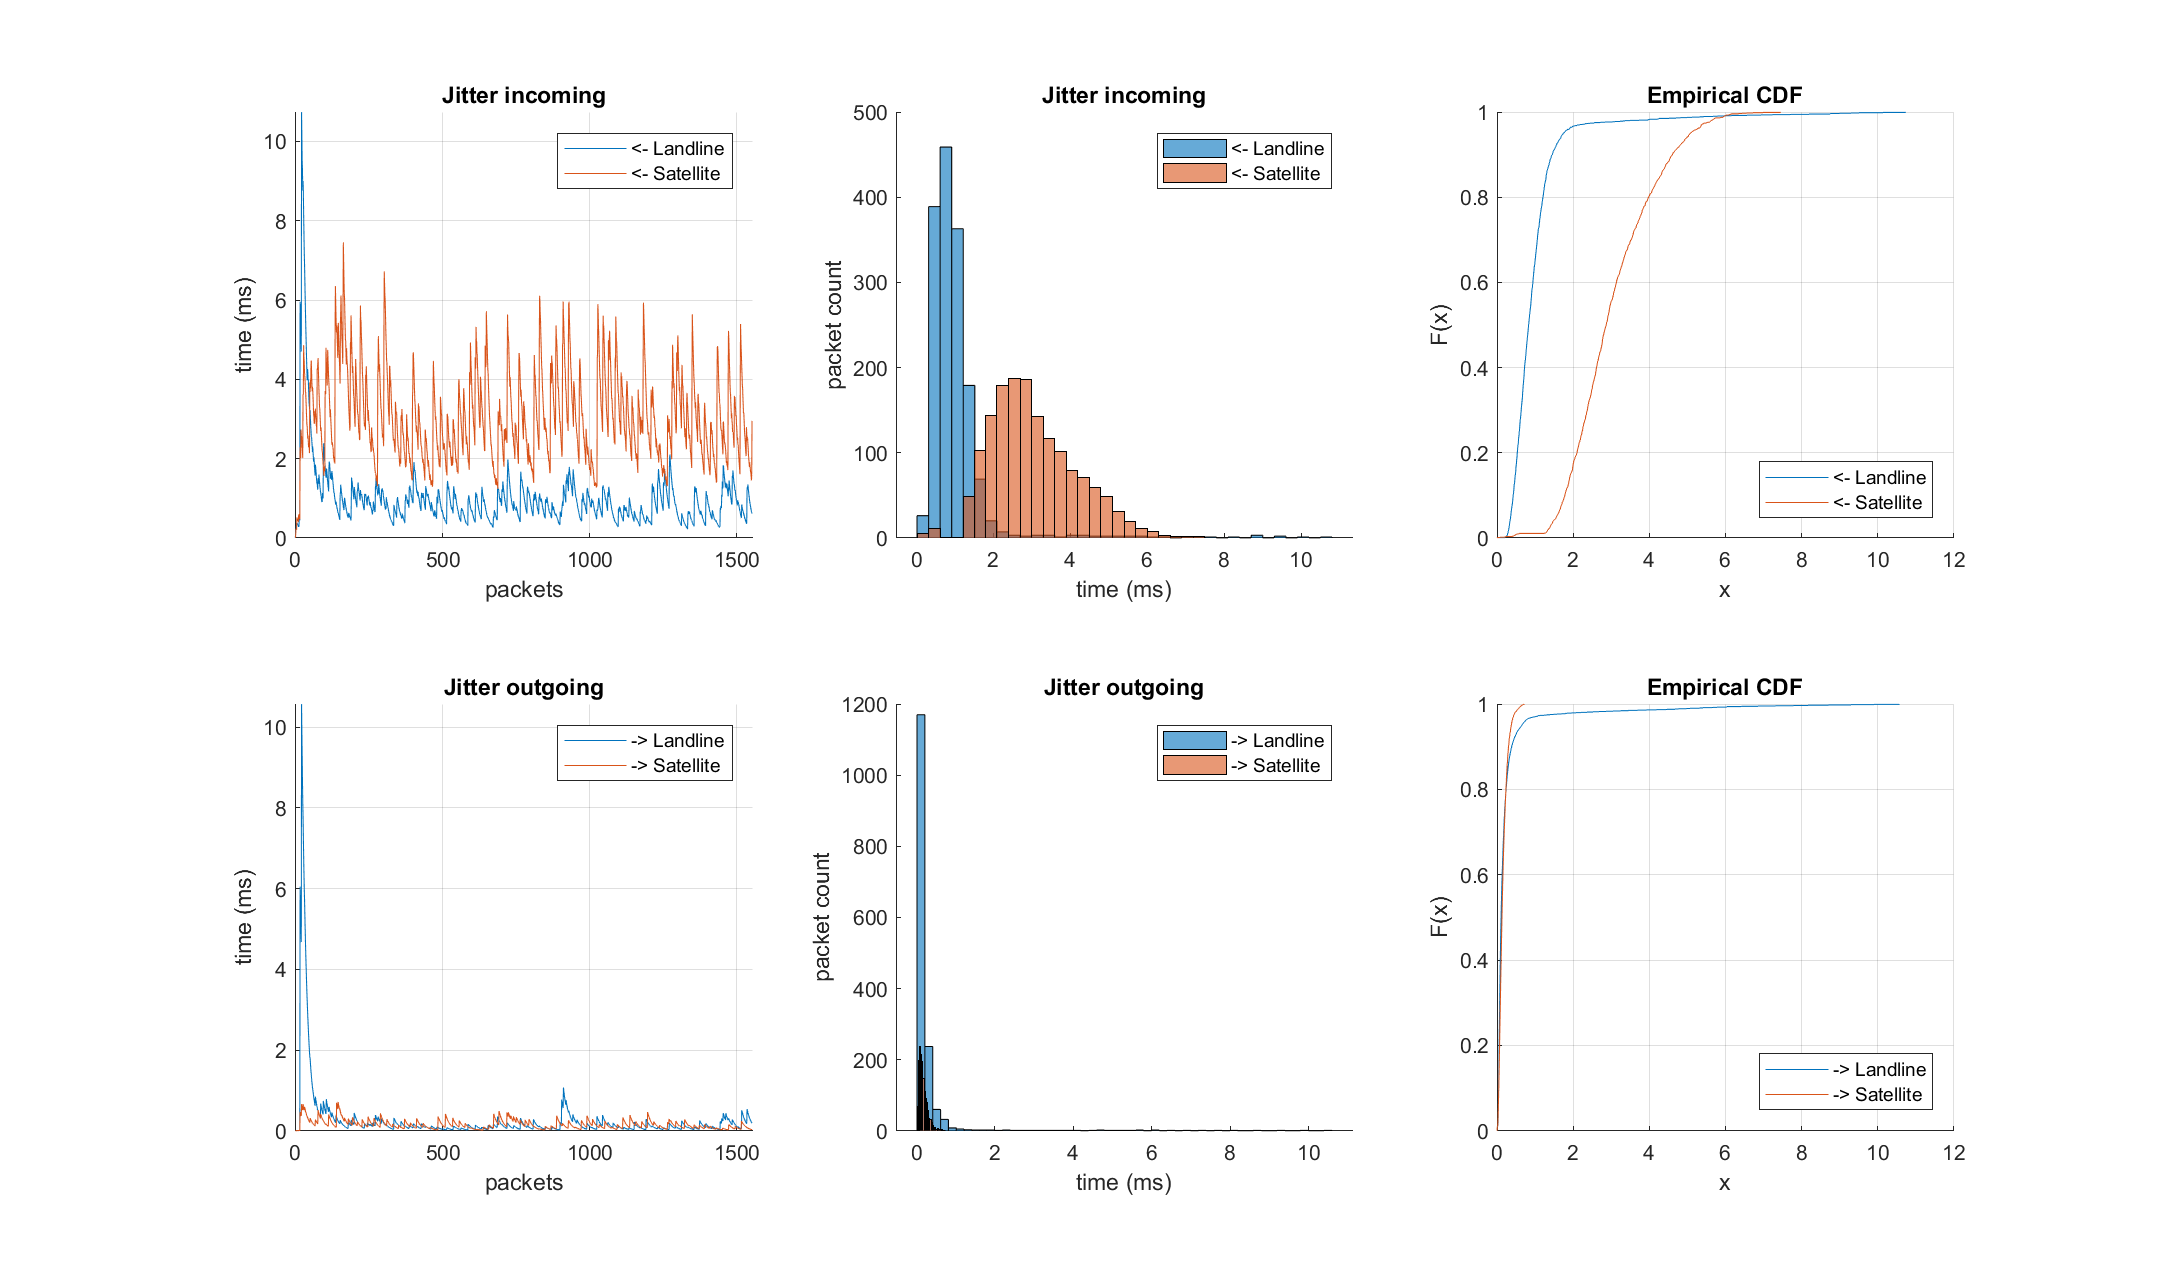
\includegraphics[width=1\textwidth]{results/Video_VP8_Jitter.eps} 
    \caption{Video Jitter in ms using VP8 codec. }
    \label{fig:vp8_jitter}
\end{figure}

Figures \ref{fig:video_jitter} and \ref{fig:video_delay} depict CDFs for the jitter and the delay values for both servers. Apart from the generally worse parameters for the Satellite server, the \texttt{VP8} codec performs better than the \texttt{H263-1998} and \texttt{MP4V-ES} codecs in the low quality network. 

Among the audio codecs, the \texttt{Opus} codec performs because of the slightly higher values for the jitter not as good as the \texttt{Speex} and the \texttt{PCMU} codecs (Figures \ref{fig:audio_jitter} and \ref{fig:audio_delay}).

\begin{figure}
    \centering
    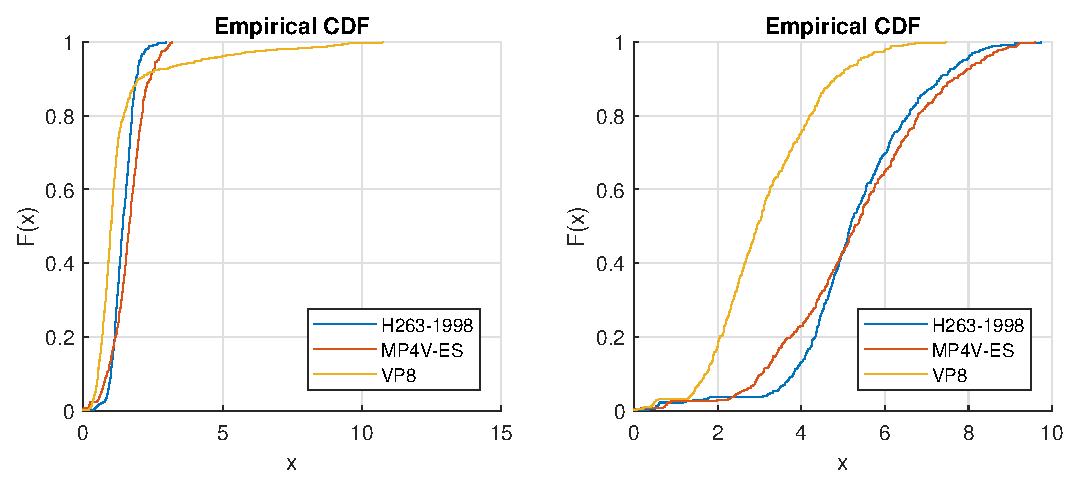
\includegraphics[width=1\textwidth]{results/Video_Codecs_Satellite_Jitter.eps} 
    \caption{Video Jitter (ms) codecs comparison for Landline (left) and Satellite (right) connections. }
    \label{fig:video_jitter}
\end{figure}

\begin{figure}
    \centering
    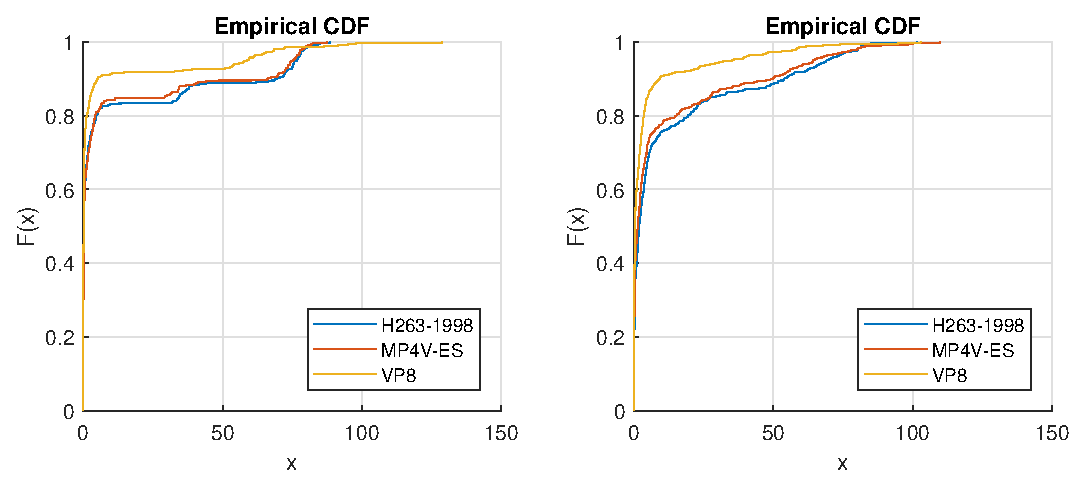
\includegraphics[width=1\textwidth]{results/Video_Codecs_Satellite_Delay.eps} 
    \caption{Video Delay (ms) codecs comparison for Landline (left) and Satellite (right) connections. }
    \label{fig:video_delay}
\end{figure}

\begin{figure}
    \centering
    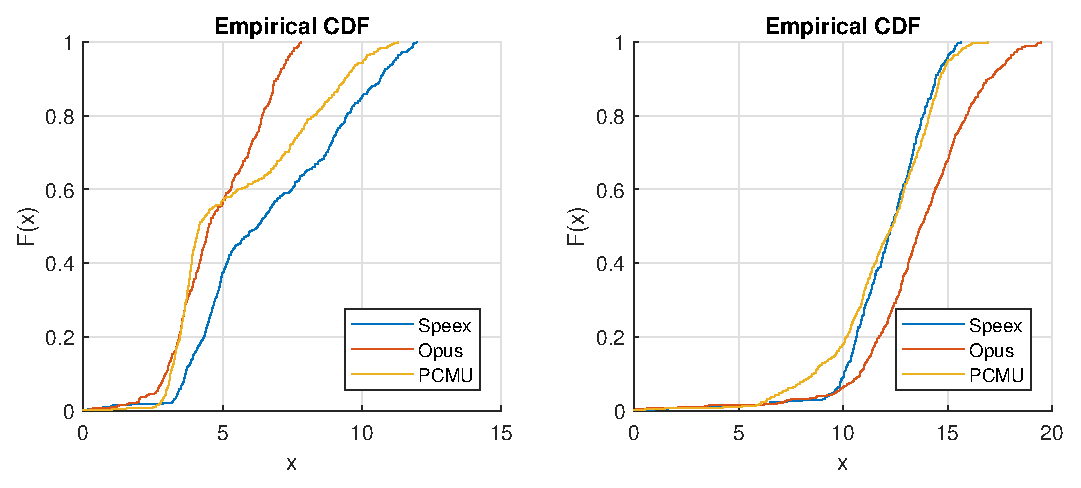
\includegraphics[width=1\textwidth]{results/Audio_Codecs_Satellite_Jitter.eps} 
    \caption{Audio Jitter (ms) codecs comparison for Landline (left) and Satellite (right) connections. }
    \label{fig:audio_jitter}
\end{figure}

\begin{figure}
    \centering
    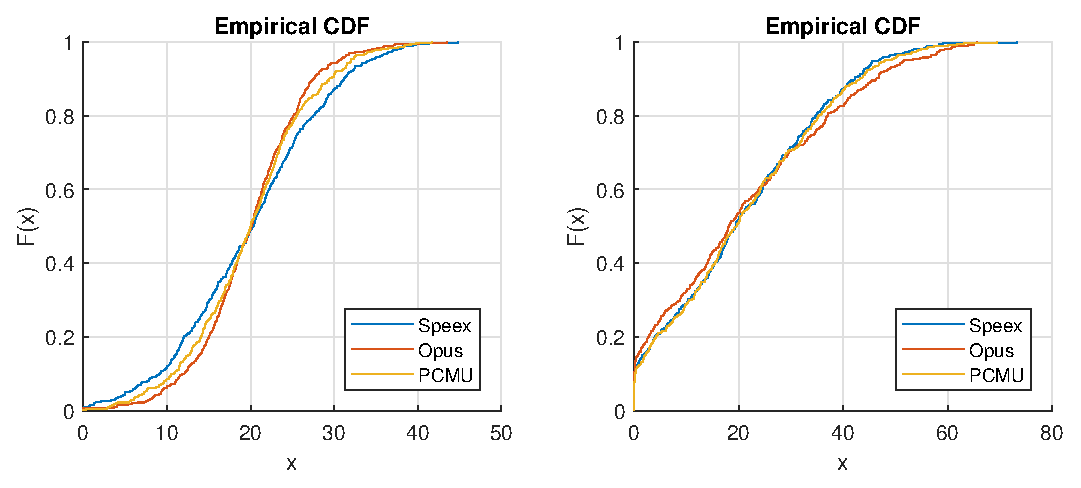
\includegraphics[width=1\textwidth]{results/Audio_Codecs_Satellite_Delay.eps} 
    \caption{Audio Delay (ms) codecs comparison for Landline (left) and Satellite (right) connections. }
    \label{fig:audio_delay}
\end{figure}

%----------------------------------------------------------------------------------------
%	SECTION X
%---------------------------------------------------------------------------------------

\bibliographystyle{unsrt}
\bibliography{references}
%%%%%%%%%%%%%%%%%%%%%%%%%%%%%%%%%%%%%%%%%%%%%%%
\end{document}
